\chapter{Introduction}

	\section{Introduction}
	\label{sec:intro}
	
	Multiparametric imaging is very important in cancer imaging. It allows the cross-correlation of observations at tumour level and  validation of new biomarkers against an established standard \cite{Padhani:2010hfa}. 
	%This is the goal for combined MRI and OptCT imaging of tumours. 
	Traditionally, tumour imaging has been approached from opposite ends of the resolution spectrum. Histology, using optical microscopy,  images tumour cells with resolution in the micron range. However, lengthy preparation steps and sectioning means that 3-D information is lost and \textit{in vivo} imaging is not possible. Magnetic resonance imaging (MRI) gives excellent visualisations of whole tumours \textit{in vivo} with contrast sensitive to malignant and benign tumours. However, the best resolution is of the order 100 microns so single cells cannot be resolved. This means the biological origin of contrast in MR images is not fully understood. 
	
	Optical computed tomography (CT) is a relatively new imaging modality which has the potential to bridge the gap between histology and MRI. It is the optical equivalent of x-ray CT, using mathematical reconstruction to produce cross-sectional images from projections through a sample. Samples can include embryos, tumours and entire excised tumours. The important advantage of using optical CT is its ability to give high resolution, high contrast images using optical dyes and stains common in histology. This distinguishes it from other modalities such as $\mu$-MRI.
	
	Forms of optical CT have been reported as far back as 1983 \cite{ray1983laser,kawata1990laser} %but only one projection image was used.  
	and a system similar to modern approaches was reported by Brown in 1992 \cite{Brown:1992}. 
	%A key point is the use of matching fluid  and sample clarification.
	%ncleared a sample of stained cochlea in 3BB:5MS. 600nm illumination to reduce scatter. 1.92mm radius imaged with resolution 16$\mu$m. But Brown is not referenced by either Gore or Sharpe. :(
	However, the field of optical CT has only significantly  progressed recently, starting in 1996 with Gore in the area of dosimetry  \cite{Gore:1999tg}. Later Sharpe developed a similar system in the area of biomedical microscopy, calling his technique optical projection tomography (OPT)  \cite{Sharpe:2002jp}. The availability of reasonably priced cameras and more computer power has meant that optical CT systems can be built relatively cheaply. This is yet another advantage over MRI scanners which are very expensive and time consuming to use.
	
	Having the ability to co-register MR images with high resolution, unsectioned optical images  is of significant  interest in cancer research. Understanding the origin of MR contrast on a cellular level would give MR the potential to be used more effectively in screening potential new drugs. optical CT also offers the chance to monitor tumour development in 3-D with fluorescent markers. These developments could be of significant help  in cancer imaging and treatment.
	
	
	%From meeting 13/12/12: mention problem with MR, fundamental limit on resolution, diffusion limit on protons. SNR. See papers by Paul Glover, Nottingham (micropscopy + limits of MR)
	
	
	
	%\newpage
	\section{Optical CT theory}
	\label{sec:theory}
	
	%The theory behind CT reconstruction is broadly the same between x-ray CT and OptCT. One minor difference is that it is common in x-ray CT for the detectors to rotate around the sample whereas in OptCT the sample rotates and the detectors are stationary. This introduces a minus sign at one stage of the reconstruction algorithm. [WHY IS THIS?]
	
	
	
	\subsection{Radon Space}
	
	When light passes through a substance, it is assumed to be attenuated by some small amount of intensity $\Delta I$ over a small distance $\Delta y$ 
	\begin{equation}
	\dfrac{\Delta I}{I} = -\mu(y)\Delta y
	\end{equation}
	where $\mu(y)$ is the linear attenuation coefficient.
	Taking the infinitesimal limit and integrating, 
	\begin{equation}
	\int_{I_0}^{I} \frac{1}{I}\, \mathrm{d}I = - \int_L \mu(y)\, \mathrm{d}y
	\end{equation}
	this leads to Beer's Law 
	\begin{equation}
	I(y) = I_{o}(y)\mathrm{e}^{-\int_L \mu(y)\, \mathrm{d}y}
	\label{eq:Beer}
	\end{equation}
	where $I_0$ is the intensity with no attenuation and $I(y)$ is the intensity at depth $y$. $L$ is the path the light ray has followed. The integral in the exponential term of Beer's Law takes into account the differences in attenuation coefficient along the path $L$. 
	
	From equation~(\ref{eq:Beer}) it is apparent that  the  intensity of a light beam after passing through a sample gives information about the line integral of the function $\mu$  along the line $L$. The CT scanning process records this information for many lines $L$ at different lateral positions and it is from this information that we reconstruct a map of $\mu$. \cite{natterer2001mathematics}
	The Radon transform maps a function into a set of its line integrals. Therefore, CT reconstruction involves an inverse Radon transform.
	
	
	
	To build  a 2-D map of attenuation coefficients, line integrals must be measured from multiple angles (see Figure~\ref{fig:projection}). If the sample rotates by some angle $\phi$ then the attenuation seen at position $(x, y)$  changes.
	The Radon transform, often called a projection or a view, is defined as
	\begin{equation}
	P_{\phi}(x) = \int\limits_{sample} \mu(x',y')\, \mathrm{d}y = -\ln\left(\frac{I_{\phi}(x)}{I_0}\right)
	\end{equation}
	where 
	\begin{equation}
	\begin{aligned}
	x' = x\cos\phi + y\sin\phi \\
	y' = -x\sin\phi + y\cos\phi
	\end{aligned}
	\end{equation}
	
	The projection information is stored in what is known as `Radon space' with dimensions $(x, \phi)$. Radon space is filled by measuring the projection value for all combinations of $x$ and $\phi$. A filled Radon space diagram is often referred to as a sinogram (see Figure~\ref{fig:sinogram}).
	
	In practice, the finite number of lines $L$ limits the resolution of reconstructions. There are two geometries for 2-D reconstructions; parallel beam and fan beam. The choice of scanning geometry also affects the resolution. \cite{natterer2001mathematics}
	
	\begin{figure}[H]
		\centering
		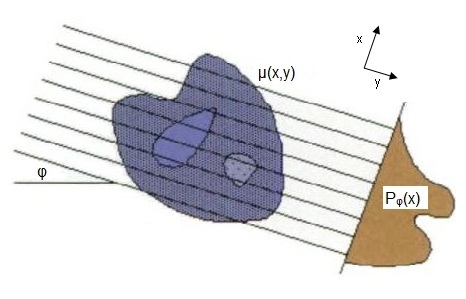
\includegraphics[scale=0.6]{intro_img/Russ_projection.jpg}
		\caption{Parallel ray geometry showing how a projection/view, $P_{\phi}(x)$, is recorded at angle $\phi$. The attenuation $\mu(x,y)$ within the sample is not uniform and projections must be taken from many angles to reconstruct a map of $\mu(x,y)$.  Here $x$ represents lateral position  and $y$ represents  depth. Figure adapted from \cite{russ2002image}.}
		\label{fig:projection}
	\end{figure}
	
	
	
	
	\begin{figure}[H]
		\centering
		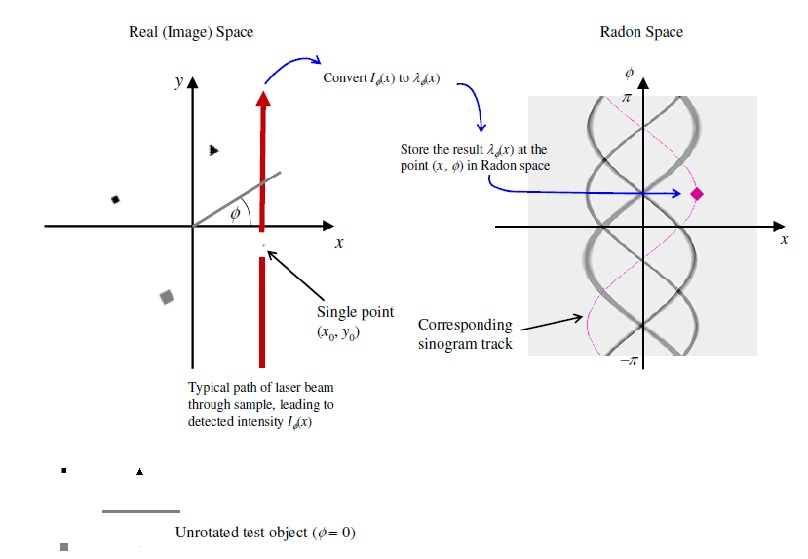
\includegraphics[width=\textwidth]{intro_img/Doran_2008_sinogram.jpg}
		\caption{Transformation from image space to Radon space demonstrated. Projection information is stored in Radon space. A 2-D image of Radon space is often called a sinogram. Different shapes produce characteristic tracks on the sinogram according to their symmetry upon rotation. Figure adapted from \cite{Doran:2008kh}.}
		\label{fig:sinogram}
	\end{figure}
	
	
	
	
	
	
	
	\subsection{Filtered Back-projection}
	\label{subsec:FBP}
	
	The information stored in a sinogram is used to reconstruct a map of attenuation within the sample. This is done through the process of back-projection.
	
	Simple back-projection involves  taking each projection point $P_{\phi}(x)$ and working back along the line integral, $L$, which created that projection in real space. Each point along $L$ is  attributed with the value $P_{\phi}(x)$. After doing this for all projection points, certain areas in real space are shaded darker as projections from different angles cross over. This builds up a picture of the shapes inside the sample. 
	
	Mathematically, back-projection can be described in terms of Fourier transforms (FTs). The 1-D FT of projection data for  angle, $\phi$, is given by
	\begin{equation}
	S_{\phi}(k_x) = \int P_{\phi}(x)\mathrm{e}^{-i x k_x}\, \mathrm{d}x
	\end{equation}
	where the FT maps $P_{\phi}(x)$ from the spatial domain to $S_{\phi}(k_x)$ in the frequency domain, also known as k-space.
	
	For the case of $\phi = 0$ this can  be written as
	\begin{align}
	S_{0}(k_x) &= \iint \mu(x,y) \mathrm{e}^{-i x k_x }\, \mathrm{d}x\mathrm{d}y \label{eq:1}\\
	&= \iint \mu(x,y) \mathrm{e}^{-i(k_xx +k_yy)}\, \mathrm{d}x\mathrm{d}y \label{eq:ky} \\ 
	&= \tilde{\mu}(k_x,k_y=0) \label{eq:3}
	\end{align}
	where $\tilde{\mu}(k_x,k_y)$ is the 2-D FT of $\mu(x,y)$.
	The extra term in (\ref{eq:ky}) is added  under the assumption that $k_y = 0$ giving $\mathrm{e}^{k_yy}=\mathrm{e}^{0}=1$. 
	
	Since the co-ordinate system can be chosen arbitrarily, equations (\ref{eq:1}-\ref{eq:3}) can be generalised for any angle $\phi$.
	This  is formalised in the Fourier Slice Theorem which states that the 2-D FT of $\mu(x,y)$ along the line at $\phi$ in k space is the same as the 1-D FT of the projection, $P_{\phi}(x)$ \cite{Doran:2008kh}.
	
	However, simple back-projection is flawed. As all the projections cross in the middle of the image, an artefact of high attenuation builds up there and edges of features in the sample are blurred.  In order to reconstruct more accurate images a mathematical trick called Filtered Back-projection (FBP) is used. 
	
	The blurring is similar to that of an out-of-focus system with point spread function (PSF) proportional to $\nicefrac{1}{f}$ where $f$ is the frequency \cite{russ2002image}. Therefore, to remove this blurring effect the image should be multiplied by the inverse of the blurring function in frequency space.
	
	The formula for reconstructing $\mu(x,y)$ using FBP involves a 2-D inverse FT of $S_{\phi}(k)$
	\begin{equation}
	\mu(x,y) = \frac{1}{2\pi} \iint \tilde{\mu}(k_x,k_y) \mathrm{e}^{i\left(k_xx+k_yy\right)}\, \mathrm{d}k_x\mathrm{d}k_y
	\end{equation}
	Converting to polar coordinates where $k_x=k\cos\phi$ and $k_y=k\sin\phi$ gives
	\begin{align}
	\mu(x,y) &= \frac{1}{2\pi} \int\limits_0^{2\pi} \int\limits_0^{\infty} \tilde{\mu}(k,\phi) \mathrm{e}^{ik\left(x\cos\phi+y\sin\phi\right)}k\, \mathrm{d}k\mathrm{d}\phi \\
	&= \frac{1}{2\pi} \int\limits_0^{2\pi}\left[\int\limits_0^{\infty}S_{\phi}(k)\mathrm{e}^{ikx'}k\, \mathrm{d}k \right]\, \mathrm{d}\phi \\
	&= \frac{1}{2\pi} \int\limits_0^{2\pi}Q_{\phi}(x')\, \mathrm{d}\phi
	\end{align}
	where $Q_{\phi}(x')$ is the projection filtered by in the frequency domain by multiplication with $k$. This is known as the ideal inverse filter, giving high weighting to high frequency components but low weighting to low frequencies. Other commonly used filters include the Hann,  Hamming, Butterworth, Shepp-Logan and Ram-Lak. Choice of filter can affect the quality of reconstructions \cite{russ2002image}.
	
	In order to use  FBP to reconstruct projections from optical CT two requirements of the Fourier Slice theorem must be satisfied. The first is that projections should be the result of rays travelling parallel to the optical axis through the sample. The second is that all points along a projection should contribute with the same weighting to the signal \cite{Wang:2007}. Optical CT design considerations focus on satisfying these requirements to obtain high quality images.
	
	
	
	%Computational methods for improving reconstructions in OPT by Birk in 2011 \cite{Birk:2011}
	
	
	
	\subsection{Optics}
	
	The quality of reconstructed images is primarily limited by the quality of projection data. There are many aspects of FBP which can degrade image quality, such as the choice of filter and the number of projection angles acquired. However, there is also a fundamental limit on resolution achievable due to the optics of the system. Unlike x-ray CT, many optical CT systems use focusing optics to acquire projections. The type of optics used in optical CT has developed over the years, different set-ups are discussed in Sections~\ref{sec:dos} and~\ref{sec:tissue}. 
	
	The Rayleigh criterion states that two objects are just resolved when the centre of one Airy disk falls on the first minimum of the other object's pattern \cite{hecht2002optics}.
	Lateral resolution is given by this distance,
	\begin{equation}
	\Delta x=r_{Airy} = \dfrac{0.61n\lambda}{\rm{NA}}
	\label{eq:res}
	\end{equation}
	where $r_{Airy}$ is the radius of the Airy function. $n$ is the refractive index of the medium around the lens, $\lambda$ is the wavelength of light and NA$=n\sin \theta_{max}$ is the numerical aperture of the lens where $\theta_{max}$ is the acceptance angle of the optics.
	
	The depth of field (DOF) is the depth within the sample over which the image is acceptably sharp while the detector is kept in a constant position . At high NA the DOF is determined by wave optics while at low NA it is dominated by the geometrical `circle of confusion' \cite{shinya1997video}. Overall, the DOF can be expressed as a sum of these two effects
	\begin{equation}
	DOF = n_{bath}\left(\dfrac{n\lambda}{\rm{NA}^{2}} + \dfrac{n}{M\rm{NA}}e\right)
	\end{equation}
	where e is the pixel size of the CCD, $n_{bath}$ is the refractive index of the medium surrounding the specimen and $M$ is the lateral magnification.
	
	According to Nyquist, the Airy disc must be sampled more than twice per DOF distance to avoid aliasing \cite{Walls:2007jl}. This constrains the detector spacing to
	\begin{equation}
	e \leq M \dfrac{r_{Airy}}{2}
	\end{equation}
	so the maximum possible DOF is given by
	\begin{equation}
	DOF_{max} = n_{bath}\left(\dfrac{1.305\lambda}{\mathrm{NA}^{2}}\right)
	\label{eq:DOFmax}
	\end{equation}
	
	Comparing equations~(\ref{eq:res}) and (\ref{eq:DOFmax}) it can be seen that the choice of NA is very important.  Choosing a large NA will give high resolution however, the DOF will be limited. The NA has a more significant effect on DOF, having an inverse square relationship. To satisfy the second requirement of the Fourier Slice theorem, projection data should only be collected from regions within the DOF. If other regions are sampled they will have less weighting being less sharply focused. 
	
	Choosing the optimum NA will depend on the sample being imaged and as a rule, high resolution imaging is limited to small samples. Some methods to overcome this DOF barrier have been proposed by different groups and include, scanning the DOF through the sample \cite{Fauver:2005} and positioning the focal plane so only half of the sample is within  the DOF at one time and then taking $360^{\circ}$ worth of projections \cite{Sharpe:2002jp}. The advantages and disadvantages of these systems are discussed further in Section~\ref{subsec:OPT}.
	
	
	
	%\subsection{Common artefacts}
	
	%Axis of rotation problems. Corrections suggested by many groups. Recently by Dong in 2012 \cite{Dong:2012}  discuss method.
	
	%Walls 2005 \textit{Noise is Poisson distributed below 2\% on an averaged signal. Therefore artefactual effects must be kept below 1\%}
	
	%Ring artefacts are generated when a feature not associated with the dosimeter sample is present in the same place in all projections. A typical cause might be a bubble or scratch on the wall of the tank containing the matching liquid. (Directly from Doran 2008)
	
	%\newpage
	\section{Development of optical CT scanning}
	
	\subsection{Dosimetry}
	\label{sec:dos}
	\subsection*{Laser scanning configuration}
	
	One of the first reported optical CT systems was developed in the area of gel dosimetry. Accurate 3-D measurement of dose delivery in radiotherapy is extremely important in developing safe treatment plans. Specialist polymer gels, such as BANG\textsuperscript{\textregistered} \cite{Maryanski:1996}, respond to irradiation with changes in optical attenuation and scattering properties.  This makes them ideal for measuring 3-D dose distributions. Previously the irradiated gels were measured by MRI and x-ray CT. However, these are expensive imaging modalities. In 1996, Gore and Maryanski published the first system for scanning polymer gels using optical computed tomography \cite{Gore:1999tg}. In later comparisons, OptCT has been found to be more precise, have reduced noise and smoother line profiles than MRI for gel dosimetry \cite{Oldham:2001gs}, although these results have since been disputed. 
	
	Gore's system consisted of a  He-Ne laser source and large area photo-diode detector (see Figure~\ref{fig:gore_setup}). Translate-rotate acquisition was employed whereby the sample was rotated and projection data  acquired  by the photo-diode over $360^{\circ}$. Small angular steps between projections are necessary for high quality reconstruction \cite{russ2002image}. For a 2-D reconstruction, projections are acquired across a slice of the sample by translating the laser beam with mirrors. For 3-D information, the sample height  had to be manually adjusted and many 2-D slices acquired. This meant scanning an entire sample took  hours and lengthy scanning times are the chief disadvantage of the laser scanning method.  Accuracy of 5\% is reported and spatial resolution of 2mm, which is roughly the same as the laser beam width \cite{Gore:1999tg}.
	
	The idea of optical CT scanning in dosimetry was quickly developed by other groups. Laser scanning set-ups were published in 1996 by \cite{Tarte:2006} and  \cite{Kelly:1998}.
	%\textit{Can't find the paper 1996 Kelly references in 1998 Med Phys says it doesn't exist.}
	Kelly \textit{et al.} claim to have independently developed their scanner which is very similar to that of Gore's. In  both Kelly's and Tarte's  scanners, the sample is rotated and translated using a stage whereas Gore used mirrors to translate the laser spot across the sample. 
	
	
	A commercial laser scanning optical CT system, OCTOPUS\texttrademark by MGS Research, Inc.
	(Madison, CT),  is an extension of Gore's original set-up with the addition of a platform capable of vertical movement for automated slice-selection \cite{Islam:2003gs}. For a number of years it was the only commercially available system and has been characterised by several groups \cite{Xu:2003cc, Islam:2003gs, Xu:2004iv, Sakhalkar:2009hb}. According to Oldham, characterisation of optical CT systems should include checks on geometric distortion, accuracy of reconstruction, scatter artefacts and reflection and refraction artefacts \cite{Oldham:2004cj}.
	
	
	
	
	%Upgraded laser Oldham 2004b \cite{Oldham:2004bv} - field photodiode mounted on a scanning arm to maintain constant distance between laser and detector. Check Oldham 2006 \cite{Oldham:2007eu}
	
	\begin{figure}[H]
		\centering
		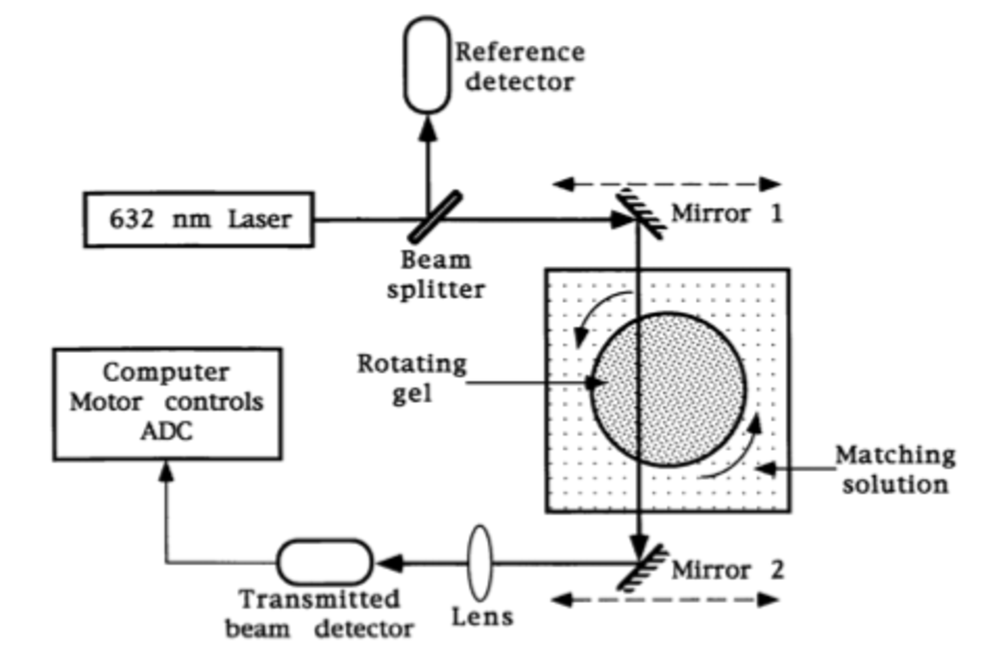
\includegraphics[scale=0.6]{intro_img/Gore_setup.pdf}
		\caption{A first generation,  Laser Scanning optical CT system developed by Gore. The sample is rotated and projections recorded at a number of angles. The  mirrors scan the laser beam across the sample but movement in the vertical direction is by manual adjustment only Figure adapted from \cite{Gore:1999tg}. }
		\label{fig:gore_setup}
	\end{figure}
	
	
	Laser scanning systems include a  beam splitter before the sample to create a reference beam. Dividing projections by the reference intensity  corrects for laser beam intensity fluctuations \cite{Gore:1999tg}.
	
	Refraction and reflection at container walls are significant concerns for all configurations of  optical CT. Generally, laser beams are incident on the gel container at a small angle, such as $5^{\circ}$, to avoid large reflection at the interface. The gel container is usually placed in a tank containing `matching fluid' with a refractive index close to that of the gel. This prevents significant refraction as the light passes into the gel. Doran found through ray tracing simulations that the refractive index of the walls of the matching tank and  gel container are not important compared to the gel and matching fluid. The optimum difference in refractive index between these two was interestingly found to be non-zero \cite{Doran:2001ee}. 
	
	To maximise the dynamic range of the system, coloured dye is commonly added to the matching fluid so the optical density of the matching fluid and gel are very similar \cite{Krstajic:2006kna}. 
	
	
	
	
	\subsection*{Pixelated detector based systems}
	
	The first CCD based optical CT system was developed in a separate field in 1996, investigating self-organising chemical structures \cite{Winfree:1996}.
	In 1997 it was adopted for dosimetry by \cite{Tarte:2007} who employed an incoherent white light source and CCD camera detection. The advantage  of a pixelated detector based system  is that an entire 2-D projection can be imaged at once, potentially increasing the scanning speed by several  orders of magnitude depending on the data through-put rate. Tarte's system used a divergent light source and diffusing screen to measure optical density in a thin gel section (see Figure~\ref{fig:tarte_ccd_setup}). 
	%For a very thin sample this adequate however, more sophisticated optics are required for bigger samples. \textbf{Does tarte reconstruct at all?}
	
	\begin{figure}[H]
		\centering
		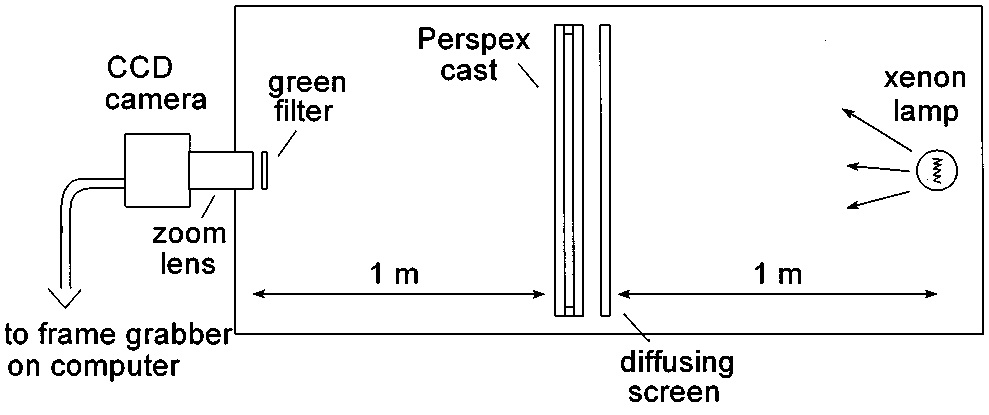
\includegraphics[scale=0.4]{intro_img/Tarte_1997_ccdsetup.jpg}
		\caption{Diagram of the first CCD-based  optical CT system for dosimetry, developed by Tarte \textit{et al.} It uses  divergent illumination from a white light source and CCD camera detection to record an entire 2D projection at once.   Figure adapted from \cite{Tarte:2007}. }
		\label{fig:tarte_ccd_setup}
	\end{figure}
	
	
	The accuracy of Tarte's system  was checked by comparison with the standard measure of dosimetry, the parallel plate ionisation chamber. It was found to be on average within 3\% of the value from the ionisation chamber \cite{Tarte:2007}. A comparison between Tarte's laser scanning and CCD set-ups found that they had similar spatial resolutions. The CCD method had improved speed of acquisition but suffered from consistently worse SNR as a photodiode detector can collect many more photons per `pixel' than a CCD camera \cite{Tarte:2007}.
	
	%The laser system 'pixel' is defined by the region illuminated by the laser spot while the photodiode has a much larger area than the spot, so it collects even photons which have diverged from a straight line. 
	
	Advances in technology have meant that  high quality detectors are much more affordable. A cheaper alternative to very high quality CCD cameras is the CMOS (Complementary Metal-Oxide-Semiconductor) detector which has the potential for higher resolution and dynamic range \cite{Doran:2008kh}. Using a higher quality detector would improve many optical CT systems  in terms of scanning speed and reduced artefacts \cite{Tarte:2007, Doran:2001ee}.
	
	
	\paragraph{Parallel beam configuration:} One method to reconstruct 3-D images with a CCD or CMOS detector is to create a broad parallel beam. This allows the use of parallel reconstruction algorithms, very similar to those used for x-ray CT. Each 2-D projection image recorded corresponds to one row for every slice in the 3-D reconstruction sinogram \cite{Doran:2008kh}.
	Telecentric optics, in which the chief rays are parallel to the optical axis, are key in the design of this configuration \cite{Walls:2005ja}. Telecentric optics can be achieved either through a careful arrangement  of  a large converging lens before the sample and standard camera lens  \cite{Doran:2001ee} (see Figure~\ref{fig:doran_ccd_setup}) or through an expensive telecentric lens \cite{Sakhalkar:2008exa}. The process of forming a parallel beam results in non-uniformities in the lightfield. This is compensated for by dividing by a `correction' or `open lightfield', image which is a projection taken with no sample in the tank \cite{Doran:2001ee}.
	
	Telecentric lenses give the advantages of parallel rays and almost constant magnification throughout the sample \cite{Oldham:2007ku}. This helps to satisfy the requirements of the Fourier Slice Theorem for high quality reconstruction mentioned in Section~\ref{subsec:FBP}.
	
	
	\begin{figure}[H]
		\centering
		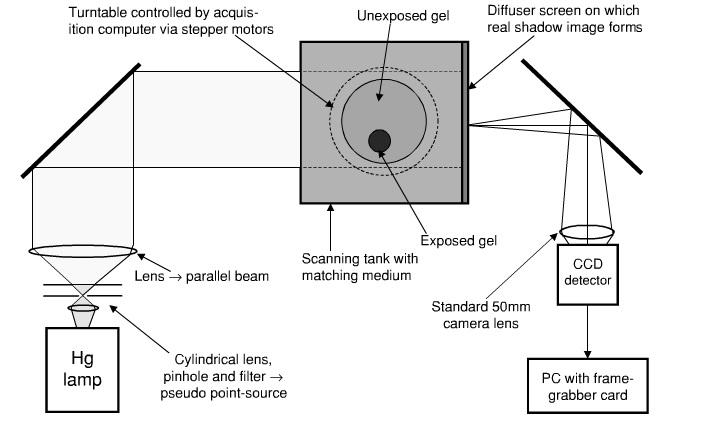
\includegraphics[scale=0.55]{intro_img/Doran_2001_ccdsetup.jpg}
		\caption{Diagram of a parallel beam  optical CT system, developed by Doran \textit{et al.} Telecentric optics create a parallel beam.  Figure adapted from \cite{Doran:2001ee}. }
		\label{fig:doran_ccd_setup}
	\end{figure}
	
	
	
	Initial systems  suffered from `graininess' due to the unstable gain of cheap CCD cameras and granularity of the diffusing screen \cite{Doran:2001ee}. Superior optics meant later systems did not require a diffuser and instead lenses were used to image directly onto the CCD \cite{Krstajic:2006kna}.  
	
	%Doran \textit{et al.} proposed some methods of correcting these problems. Oscillating the diffuser screen at high frequency ``\,`smears' out the granularity'' while randomly horizontally displacing the CCD camera by a few pixels  between acquisitions can reduce the effect of `bad'  pixels \cite{Doran:2001ee}.
	% The parallel configuration appears to be more susceptible to schlieren artefacts caused by refractive index inhomogeneities in the sample \cite{Krstajic:2007hk}.
	
	
	
	
	
	
	\paragraph{Cone beam configuration:}
	Wolodzko \textit{et al.} published the first cone beam optical CT system with CCD detection for gel dosimetry \cite{Wolodzko:1999}. One advantage of this configuration is the optics for producing a cone beam are much simpler than those for producing accurate parallel beams \cite{Doran:2008kh}. However, the reconstruction is computationally more complex \cite{hsieh2003computed}. A commercial cone-beam system, Vista\texttrademark by Modus Medical Devices Inc. (London, ON, Canada),  is available and reviewed recently by Olding \textit{et al.} \cite{Olding:2011eta}.
	
	
	\begin{figure}[H]
		\centering
		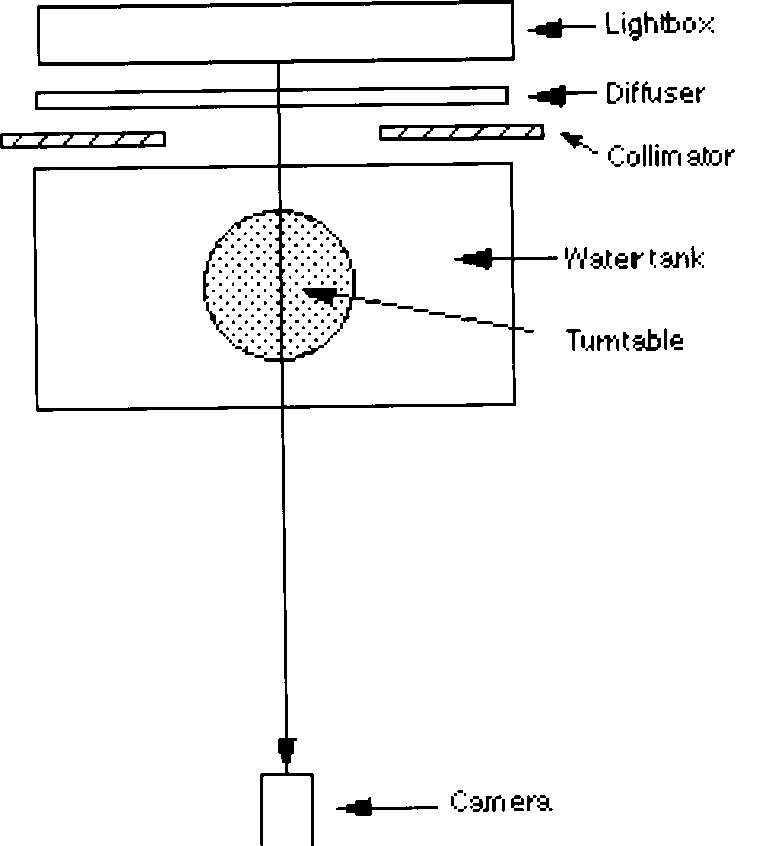
\includegraphics[scale=0.3]{intro_img/Wolodzko_1999_conesetup.jpg}
		\caption{The first cone-beam CCD configuration for optical CT. The optics are much simpler than for parallel beam systems. Figure adapted from \cite{Wolodzko:1999}.}
	\end{figure}
	
	
	There has not been experimental comparison of parallel and cone-beam systems. However,  Doran suggests that while cone-beam is usually somewhat cheaper due to simplified optics, modern parallel-beam systems have better scatter-rejection and may have fewer stray light problems \cite{Doran:2008kh, Olding:2011eta, Thomas:2011eja}.
	
	
	
	
	
	
	
	
	
	
	%Refraction and reflection at container walls are significant concerns for all configuration of dosimetry with OptCT. These problems have been investigated with Mie theory modelling of light paths. Doran found through ray tracing simulations that the refractive index of the walls of the matching tank and  gel container are not important compared to the gel and matching fluid. The optimum difference in refractive index between these two was calculated to be 0.0025 and not zero as originally thought.\cite{Doran:2001ee} Another counter intuitive finding was that the ideal gel container wall thickness is not the thinnest possible but some median thickness which 
	
	%Problems with vial walls misrepresentation due to refractive index mismatch. \cite{Doran:2001ee}
	
	%Illumination is chosen based on the configuration used and the wavelength range which is optimum for dose measurement.  
	%Stray light minimisation is very important in OptCT. Dark room, shield the illumination source. Interference filters. REF 
	
	
	%Repeatability of experiments, have locking method for samples. REF
	%Centre of rotation recovery, mostly post-processing. In theory section. 			
	
	%\textit{The first is laser based and has several design considerations including minimisation of interference effects and stray light; scatter from optical components and the radiochromic gels themselves, reflection; dynamic range; wavelength selection; wall corrections plasma discharge from lasers; temperature changes; and the characterisation of detectors.A general disadvantage of scanners based on pixelated detectors together with a wide beam is the possible introduction of artefacts by refractive index inhomogeneities (schlieren). } from \cite{Doran:2008kh}
	
	
	
	
	
	
	
	%\newpage
	\subsection{Tissue imaging}
	\label{sec:tissue}
	\subsection*{Optical Projection Tomography}
	\label{subsec:OPT}
	Another version of optical CT was  developed by Sharpe \textit{et al.} in the area of 3-D microscopy for gene expression studies \cite{Sharpe:2002jp}. Although this set-up in 2002 came after Gore's they are apparently independent and Sharpe named his technique Optical Projection Tomography (OPT).
	
	Although other techniques for 3-D microscopy are well established, OPT offers some unique advantages. 
	Confocal microscopy offers high resolution images up to a depth of about 1 mm \cite{Webb:1996}. However, it is limited to fluorescent signals meaning many optical stains used routinely in histology would not work. Optical coherence tomography (OCT), which is commonly used in ophthalmology, is capable of micrometer-scale resolution but with  depth limited to 2--3 mm in tissue \cite{huang1993optical}. Both of these techniques generate tomographic images through sectioning whereas OPT is a projection based tomography technique \cite{Sharpe:2003cm}. Avoiding sectioning is important in producing truly representative 3-D images \cite{Oldham:2007ku}. Another advantage of  OPT is its ability to  image much larger specimen, with depth of around 3 cm being reported \cite{Oldham:2007ku}. This superior imaging depth not just due to clarification of the samples, discussed in Section~\ref{sec:clearing}. OCT and confocal systems have also been tested with clearing agents and the reported gains in depth vary between 20-150\% in OCT \cite{Tuchin:2002} which is significantly shallower than optical CT.
	
	
	Sharpe's original system uses a microscope to focus projections of a mouse embryo onto a camera imaging chip.  Sharpe reports some impressive images as reproduced in Figure~\ref{fig:SharpeOPT}. Use of the microscope gives resolution of about 5--10 $\mu$m meaning single-cell membranes, around 10 $\mu$m thick, can be seen\cite{Sharpe:2002jp}. However, the high NA  optics which give high resolution limit the DOF. Sharpe decided to circumvent the problem of a low DOF by positioning the rotational axis so only half the specimen was in focus at once. $360^{\circ}$ of projections were taken to collect in-focus data from all points. The problem with only having half of specimen in focus at once is that unfocused light is superimposed upon the focused data and included in the reconstruction. This leads to blurring, which is worse with distance from the axis of rotation. Walls \textit{et al.} proposed a method of correcting this defocusing effect using a frequency-distance filter, as described by Xia for SPECT \cite{xia1995fourier,Walls:2007jl}. The filter narrows the PSF to in-focus data allowing in-focus, high resolution images to be reconstructed \cite{Walls:2007jl}.
	
	
	
	In dosimetry the refractive index within the polymer gels is roughly uniform. In tissue this is not the case, with scattering and refraction occurring at cell membrane interfaces. To make high resolution reconstruction through back projection possible, light paths through the specimen must be able to  be approximated as parallel line integrals meaning refraction must be minimised. A process called optical clearing or clarification is employed which renders tissue optically transparent. An optical clearing agent (OCA) replaces the lower refractive index intra-cellular fluid. It acts as a matching fluid within the sample itself. The mechanism for this differs between agents, see Section~\ref{sec:clearing} for more detail. 
	
	
	
	
	
	\begin{figure}[H]
		\centering
		\subfigure[OPT setup]{\label{subfig:OPTsetup}
			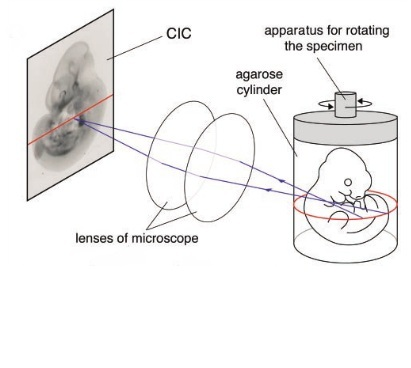
\includegraphics[width=0.5\textwidth]{intro_img/Sharpe_2002_setup.jpg}}
		\subfigure[Mouse images]{\label{subfig:OPTmouse}
			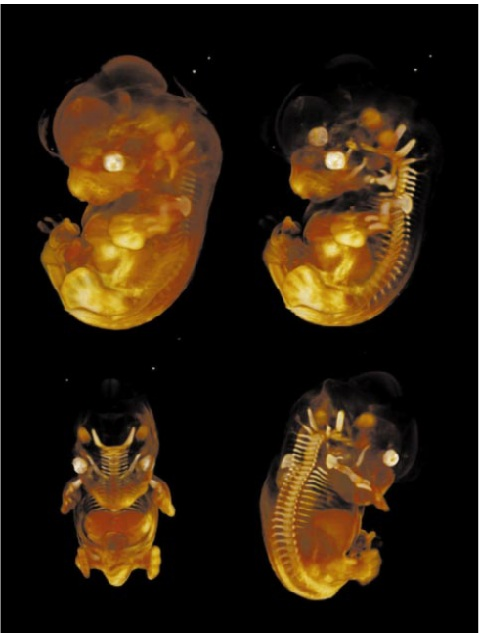
\includegraphics[scale=0.5]{intro_img/Sharpe_2003_mouse.jpg}}
		\caption{Part (a) shows the optical set-up for the first OPT system by Sharpe. CIC indicates the camera imaging chip. A microscope is used to focus projection images onto the CIC. The specimen is set in agarose gel for stability. Figure adapted from \cite{Sharpe:2002jp}. Part (b) shows some false colour images of a TS21 mouse embryo stained with alcian blue and imaged with OPT. The images have varying degrees of opacity allowing control of which internal organs are seen. Figure  adapted from \cite{Sharpe:2003cm}.}
		\label{fig:SharpeOPT}
	\end{figure}
	
	
	
	
	In 2005 Fauver reported a modified version of OPT capable of imaging single cell nuclei with 0.9$\mu$m resolution (see Figure~\ref{fig:fauver_setup})\cite{Fauver:2005}. The OPT microscope includes a rotation stage and  piezoelectrically driven objective lens. In a technique similar to Hausler \cite{hausler1972method} the objective lens is scanned axially to create an extended DOF image which is also known as a pseudo-projection. The extended DOF means features have the same focus from all angles, allowing high resolution reconstruction. However, this is not a truly quantitative technique, hence pseudo and not true projections are recorded. A high NA lens gives high resolution at the expense of low depth of field. If such high resolution is not required, lower NA optics would be a more quantitative way to generate  projections than scanning a high NA lens.
	
	
	
	\begin{figure}[H]
		\centering
		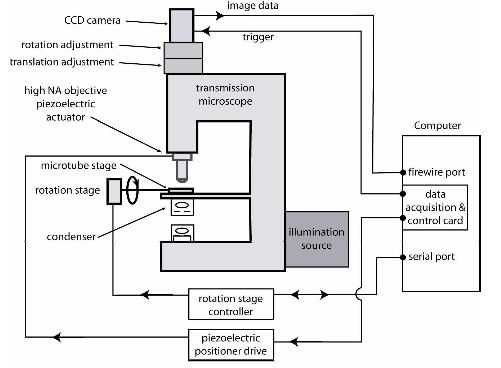
\includegraphics[scale=0.8]{intro_img/Fauver_2005_setup.jpg}
		\caption{OPT microscope for imaging single cell nuclei. A microcapillary tube injected with cells is rotated with sub-micron precision. The piezoelectric objective lens is scanned axially to create extended depth of field images. Figure adapted from \cite{Fauver:2005}.}
		\label{fig:fauver_setup}
	\end{figure}
	
	
	Wang and Wang have reported an improvement to OPT giving higher axial and lateral resolution, even for slices far from the optical axis \cite{Wang:2006hy, Wang:2007}. As previously mentioned, to obtain high quality reconstructions the projections should closely approximate a line integral of parallel rays passing through the sample \cite{Wang:2006hy}. This is not exactly the case for  OPT, which limits the best resolution possible. Wang proposed placing an iris at the back focus of the objective lens. This reduces divergence of the projection rays from paths parallel to the optical axis giving qualitatively better resolution.
	
	
	\subsection*{Fluorescent/emission  optical CT}
	\label{subsec:eOPT}
	
	Sharpe was the first to identify the possibility of using OPT to image fluorescent stains in biological specimen \cite{Sharpe:2002jp}. There are a wide range of fluorescent optical stains in use in histology making this development particularly useful for biological imaging. It also offers the advantage of being able to record multiple signals independently unlike  transmission OPT (tOPT) \cite{Sharpe:2002jp}. 
	
	%Include a paragraph on terminology? OPT and OptCT seem to be able to be used almost interchangeably in later tissue imaging papers. Need to pick one name and explain other groups use other terminology.
	
	Optical emission CT (OptECT) also known as emission OPT (eOPT) is the optical equivalent of SPECT (single photon emission computed tomography) \cite{Oldham:2007ku}.  Instead of measuring the attenuation of photons through a sample (like tOPT), eOPT signal comprises of fluorescence photons emitted along a ray path \cite{Walls:2005ja}.
	
	
	
	Some changes from the set-up (see Figure~\ref{fig:eOPTsetup}) from tOPT  include the addition of a narrow bandwidth excitation filter before the sample. This selects for the excitation wavelength of the fluorescent marker being used in the sample. The illumination is perpendicular to the detector to avoid detection of the illumination light rather than fluorescence. An emission filter before detector selects for the longer emission wavelength of the fluorophores, again to avoid contamination from auto-fluorescent and ambient photons being picked up by the CCD. To avoid photobleaching systems often include a shutter to turn off the lamp when not imaging.  The image forming optics is the same as for tOPT, although the reconstruction and artefacts are different \cite{Walls:2005ja}.
	
	
	
	Oldham \textit{et al.} have adapted Sharpe's eOPT set-up by changing from microscope to bench-top apparatus, similar to their dosimetry optical CT system \cite{Oldham:2006, Oldham:2007ku}. Microscope based systems suffer from poor DOF as the optics are designed to image flat samples.  Oldham's custom made set-up employs telecentric optics giving much improved DOF capable of imaging samples up to 3 cm \cite{Oldham:2007ku}. However, better DOF is achieved at the cost of worse lateral spatial resolution and this trade-off must be considered with respect to the information required from the specimen \cite{Krstajic:2006kna}.   A comparison of microscope and telecentric systems would be very interesting in future work.
	
	
	
	\begin{figure}[H]
		\centering
		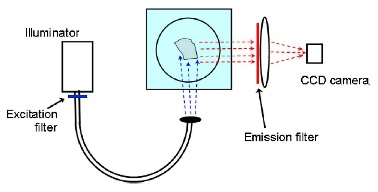
\includegraphics[scale=1]{intro_img/Oldham_2007ku_eCTsetup.jpg}
		\caption{Example of setup for OptECT/eOPT imaging. Filters are used to select for the excitation and emission wavelengths of the fluorescent stain. This set-up can give an image but no quantitative information without specialised reconstruction techniques discussed below. Figure adapted from \cite{Oldham:2007ku}.}
		\label{fig:eOPTsetup}
	\end{figure}
	
	
	
	
	
	
	
	%\subparagraph{Quantitative eOPT:} 
	There are several reasons why eOPT data is not quantitative. The most significant problem is that an unknown number of emitted photons are attenuated within the sample. This requires a mathematical model of attenuation for correction. The second problem is that some incident photons are attenuated before they can cause excitation.  This can be compensated for with simultaneous illumination from multiple angles \cite{Kim:2008eua}.  Another problem identified by Darrell \textit{et al.} is a defocusing effect caused by the lower intensity of of fluorophores positioned outside of the focal plane. Darrell's method of quantifying eOPT data involved a Fourier optics based model which accounted for the defocusing effect and isotropic emission attenuation \cite{Darrell:2008gd}. A weighting function was calculated based on this model. The function was used in FBP and acts as a window function, spreading the projection information unevenly over the reconstruction image plane.
	
	Kim \textit{et al.} have also published a method for correction of emission attenuation \cite{Kim:2008eua}. This method is similar to those used for attenuation correction in SPECT. A co-registered image from tOPT is used to construct an attenuation map and calculate attenuation-survival probabilities for the sample. The probabilities are then used in an iterative OSEM (ordered-subsets expectation-maximisation) reconstruction \cite{Kim:2008eua, hudson1994accelerated}. This attenuation correction method was tested using a  phantom with known fluorescent fibres and corrected images showed more uniform intensity across the three fibres, differing by 4\% in the corrected images but as much as 24\% in uncorrected data \cite{Kim:2008eua}.
	
	In an extension of Kim's method, Thomas \textit{et al.} were the first to report a comprehensive correction for  eOPT \cite{Thomas:2010gt}. Their iterative method corrects for both emission and excitation attenuation and non-uniformities in the light source. 
	Tests of their technique using phantoms show that it can give quantitative information of 3-D fluorophore concentration. This is could be very biologically useful, for example looking at uptake of drugs in tumour treatment. 
	
	
	
	
	
	
	%\subparagraph{Live eOPT:} 
	There have been attempts at performing OPT  on live specimen \cite{Boot:2008dt, Vinegoni:2008ix, Colas:2009}. The chief difficulties in this are developing a method limiting scatter and refraction  whilst also keeping the specimen alive. Boot and Sharpe reported their efforts for \textit{in vitro} time-lapse quantitative eOPT  imaging through tracking GFP expression of a growing mouse embryo limb bud, about 1 mm in size \cite{Boot:2008dt}. 
	Live OPT has also been used in molecular imaging tracking a changing 3-D gene expression pattern \cite{Colas:2009}.
	Vinegoni \textit{et al.} reported \textit{in vivo} imaging of Drosophila melanogaster pupae without clearing or matching fluids \cite{Vinegoni:2008ix}.  As there is no clearing involved and a mathematical model is required for reconstruction Vinegoni called this `mesoscopic' imaging rather than OPT/optical CT.  
	%A polarisation analyser in front of the CCD rejects highly scattered photons which lose their polarisation state. 
	Although gathering some biologically interesting information, the resolution was much worse than conventional OPT limiting the applications for this technique. It would be fantastic to be able to monitor tumour development in 3-D. Doing live imaging means the mouse could be its own control, instead of sacrificing many mice at different stages of tumour development. This may not be possible due to limited size and resolution.
	
	
	
	
	%Walls: Have to be careful with eOPT systems using mercury arc lamp as it suffers from fluctuations which get worse with age, as bad as 10\%. This can introduce a smearing artefact due to the high-frequency component of the fluctuations. Walls ran simulations to calculate the best way to compensate for the fluctuations using intensity measurements from the lamp itself and a Gaussian distribution for noise with sd of 1.2\% and 5\% for an older lamp. Computational method explained on page 7. Relevant?
	
	
	
	
	
	
	%\newpage
	\section{Optical Clearing}
	\label{sec:clearing}
	
	%Need for refractive index matching to ensure parallel beam assumption is true enough that we can emloy traditional reconstruction techniques. 
	Optical clearing or clarification is a very important step in optical CT imaging of tissue. Tissue is made up of many components of different refractive indices, meaning there are many optical boundaries for scatter and refraction to occur at. This is the reason why visible wavelength light does not penetrate very far in tissue. To use the parallel ray assumption  in CT reconstruction, refraction and scatter at cell membrane interfaces within the sample must be minimised \cite{Oldham:2006}.  This is accomplished with clearing.
	
	During clearing, intracellular  fluid is replaced with a optical clearing agent (OCA). There are many choices of OCA but they should all have refractive indices matching the tissue to be imaged and be hyperosmolar (i.e. have a very high solute concentration) \cite{tuchin2007tissue}.
	
	
	A very popular technique for clearing is the Optical Immersion technique. The sample is set in agarose gel for stability. The gel contains pores which allows diffusion of the OCA. The most commonly used OCAs for OPT are benzyl-alcohol-benzyl-benzoate (BABB, refractive index 1.55) or methyl salicylate (MetSal, refractive index 1.53). These are both aromatic organic solvents and are not miscible in water. Therefore a graded sequence of ethanol and OCA solutions is required to replace the intracellular water with the OCA \cite{Oldham:2006}. 
	
	Some OCAs, including glycerol and dimethyl sulfoxide (DMSO), can be directly applied to the tissue without need for graded ethanol solutions. However, they have been shown to be less effective than BABB and MetSal and cannot penetrate deeper than 1 cm \cite{Oldham:2006}.  Glycerol may be more suitable for \textit{in vivo} or live studies as it is biologically inert however DMSO would not be suitable due to high toxicity \cite{Wen:2009is}.
	
	%BABB has n=1.56 while water is n=1.33, what is n for tissue? \cite{Walls:2005ja}
	
	Glycerol appears to be the best OCA for clarification of the skin \cite{Vargas:1999, Wen:2009is}. Its refractive index (1.46) is very similar to that of collagen which is the main scatterer in skin. What is unique about glycerol is the clearing effect is reversible upon rehydration with phosphate buffered saline solution \cite{Vargas:1999}. 
	
	The mechanism for how OCAs bring about optical clarification is not clear. It was previously thought the effect was purely due to refractive index matching however some work has shown that clearing skin with alcohol doesn't correlate with the OCA's refractive index \cite{Choi:2005, Mao:2008}. Additionally, glycerol's reversibility indicates that its clarification mechanism is different to other agents. Some  proposed mechanisms include the dissociation of collagen (unravelling of the fibrous structure) and  dehydration (reducing the space between scatterers) as additional clearing effects \cite{Yeh:2003, Wen:2009is}.
	
	
	
	
	Preserving fluorescent signal is very important when clearing for eOPT/OptECT applications. Oldham and Sakhalkar have tested some clearing and fixing protocols with different fluorescent proteins \cite{Sakhalkar:2007hp, Oldham:2008dfa}. Although it is common to fix tissue samples with paraformaldehyde (PFA), it was found that this resulted in an almost complete loss of fluorescent signal. Fixation with ethanol was found to preserve fluorescence and keep fluorophores robust upon application of BABB or MetSal. Although BABB was found to give better optical clarity in general, MetSal gave better fluorescence preservation. The optimal procedure was a combination of ethanol fixation and MetSal clearing which was tested on red and green fluorescent proteins (RFP and GFP) \cite{Sakhalkar:2007hp}.
	
	
	The exact concentrations of OCA needed and the specific OCA used will depend on the tissue and form of imaging to be performed. Finding the optimum chemicals for our purpose will involve trial and error as it has been previously shown that clearing effects are unpredictable due to the complex nature of the interactions between OCA and tissue \cite{Wen:2009is}.
	
	
	
	%\newpage
	\section{Optical Staining}
	\subsection*{Staining for Cancer Markers}
	
	The goal of our investigation will be characterising MRI contrast in tumours by comparison with detailed 3-D maps of histological stains given by optical CT. Staining for tumour recognition and characterisation is a well established area for histology and will be briefly reviewed here.  One aspect to be investigated is how these stains work in the presence of OCAs. Unfortunately, Oldham has not found a method of combining immunohistological stains with clearing procedures, making \textit{in vivo} staining the most attractive option at present \cite{Oldham:2008dfa}.
	
	
	
	%Being able to use optical stains is extremely useful for computer recognition of organs, can pick better thresholds. \cite{Sharpe:2003cm}
	
	%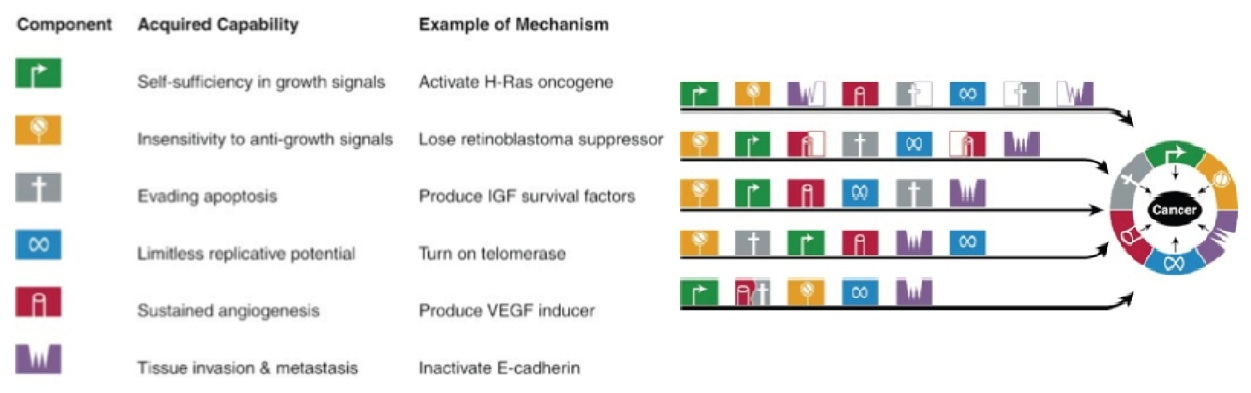
\includegraphics[scale=0.45]{Hanahan_2000_hallmarks.jpg}
	%\caption{Diagram showing the six hallmarks of cancer. These adaptations are believed to be necessary for  tumours to become macroscopic. The changes can be acquired in many different ways and in different orders chronologically, as illustrated in the diagram. Figure adapted from \cite{Hanahan:2000}}
	
	%\begin{figure}[H]
	%\centering
	%\subfigure[Traditional Hallmarks]{\label{subfig:hallmarks}
	%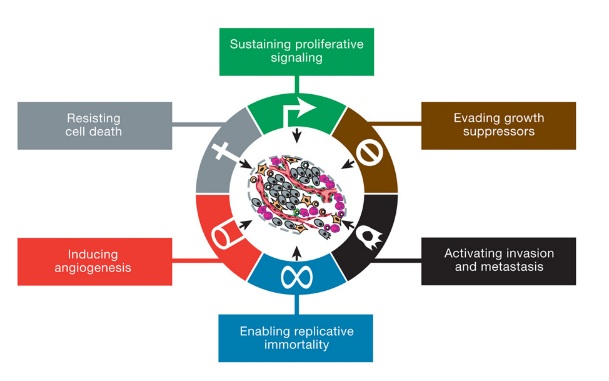
\includegraphics[width=0.45\textwidth]{Hanahan_2011_hallmarks.jpg}}
	%\subfigure[New hallmarks]{\label{subfig:newhallmarks}
	%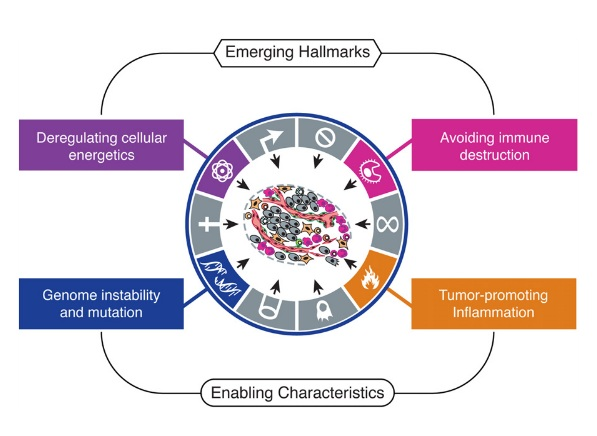
\includegraphics[width=0.45\textwidth]{Hanahan_2011_emerginghallmarks.jpg}}
	%\caption{Diagram showing the six hallmarks of cancer (\ref{subfig:hallmarks}) and some emerging characteristics that appear to also be necessary for tumours to become macroscopic (\ref{subfig:newhallmarks}). The changes can be acquired in many different ways and in different orders chronologically. Figure adapted from \cite{Hanahan:2011gua}}
	%\label{fig:hallmarks2011}
	%\end{figure}
	
	
	The primary hallmarks of cancer, which are believed to be present in virtually all tumours, are listed in Figure~\ref{fig:padhani} \cite{Hanahan:2000}. How these acquired capabilities are gained differs between individual tumours. However, there are some common pathways that can provide targets for therapy. The hallmarks also give some clues for imaging tumours (see Figure~\ref{fig:padhani}). Certain genes have been found to be very common in the route to gaining these capabilities. For example, inactivation of the p53 tumour suppressor gene is found in more than 50\% of  human tumours, giving the tumour cells the ability to evade apoptosis (programmed cell death). This gene can be tracked via reporter genes, such as HSV1-tk(GFP) which can then be imaged with positron emission tomography (PET) \cite{Doubrovin:2001}.  
	
	The area of molecular imaging is relatively new and usually involves the use of a reporter gene and complimentary reporter probe, the accumulation of which gives an indication of gene expression \cite{Blasberg:2003}. Different reporter probes can be imaged with MRI, PET, SPECT and optical techniques. Optical techniques have the advantage of being more cost and time-effective than MRI or nuclear methods. As mentioned before, optical CT has the additional advantage of better depth penetration than other common optical imaging methods such as confocal microscopy.
	
	%One such common target is the vascular endothelial growth factor (VEGF) which is often overexpressed in tumours and is important for angiogenesis. Blocking VEGF can stop additional blood flow to the tumour and restrict its growth. 
	
	%Other possible hallmarks have been identified which include evasion of anoikis (cell death signals caused by loss of cell-ECM contact) and increased glucose consumption through increased glycolysis. \cite{Gatenby:2008} 
	
	
	
	\begin{figure}[H]
		\centering
		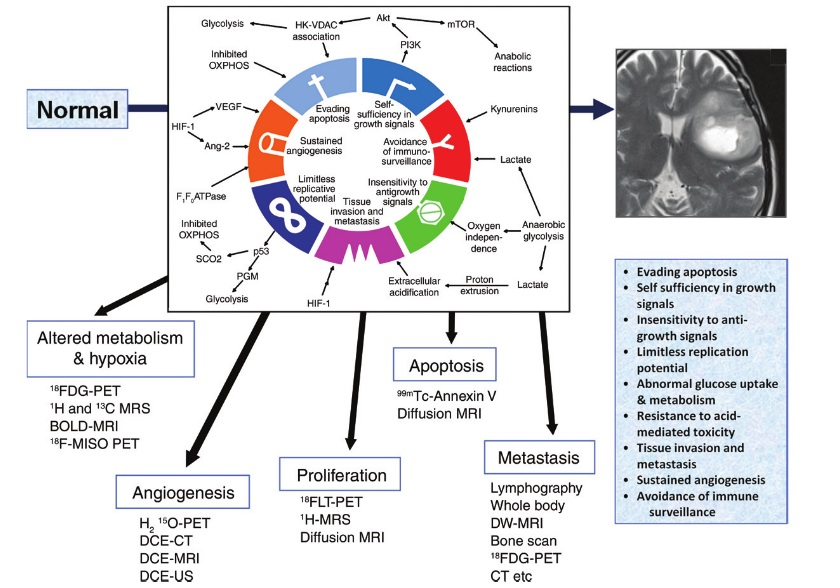
\includegraphics[scale=0.6]{intro_img/Padhani_2010_hallmarks.jpg}
		\caption{Diagram linking functional imaging modalities to the hallmarks of cancer. Figure adapted from \cite{Padhani:2010hfa}.} %\textit{DW}:diffusion weighted, \textit{DCE}:dynamic contrast agent, \textit{Bold}: blood oxygenation-level dependent,\textit{US}: Ultrasound, \textit{MRS}: magnetic resonance spectroscopy, \textit{Ang-2}: angiopoietin-2, \textit{FLT}: fluorothymidine, \textit{HK}: hexokinase, \textit{OXPHOS}: oxidative phosphorylation, \textit{PGM}: phosphoglycerate mutase, \textit{PI3K}: phosphatidylinositol 3-kinase, \textit{SCO2}: synthesis of cytochrome c oxidase 2, \textit{VDAC}: voltage-dependent anion channel. Figure adapted from \cite{Padhani:2010hfa}.}.
		\label{fig:padhani}
	\end{figure}
	
	
	Fluorescent proteins have revolutionised the area of tumour imaging, allowing real-time imaging of tumour angiogenesis, metastases, cell invasion and motility \cite{Hoffman:2005}. Using these proteins can give visualisation of a single metastatic  cell in normal tissue, far beyond the ability of histology which is the current gold standard of imaging \cite{Hoffman:2009}. The ability to colour-code cells according to genotype and phenotype is a massive advantage when monitoring the progression of tumours and their response to treatment.
	Some disadvantages of using fluorescent markers include the complication of  quantifying the data, high auto-fluorescence in the blue-green window which limits SNR, fluorophore photobleaching and high levels of scatter and attenuation of photons in tissue \cite{Gross:2005}. However, these problems are being solved as fluorescent imaging becomes more common-place. 
	
	
	The most common fluorescent marker used is  green fluorescent protein (GFP) and its spectrally shifted variants with emission ranges from 442-645nm \cite{Hoffman:2005}. The GFP gene was first cloned from \textit{Aequorea victoria} jellyfish and has since been humanised giving high expression and signal for use in mammals \cite{Hoffman:2009}. They are popular markers due to their high extinction coefficient and high quantum yield giving very bright and efficient fluorescence. The variants are spectrally different enough to can be used simultaneously, marking different aspects of the biology \cite{Hoffman:2005}. 
	
	With the discovery of red and NIR fluorophores, fluorescent optical molecular imaging is becoming  more widespread. These markers avoid the problem of blue-green autofluorescence that GFP experiences and also have slightly deeper penetration due to the therapeutic window in tissue. The first red fluorescent protein (RFP) was cloned from \textit{Discosoma} coral in the late 1990s and has been modified giving DsRed-2, a very bright protein with emission peak at 588 nm. Other longer wavelength variants have been developed such as mPlum and mCherry however these are less bright \cite{Hoffman:2009}. A newer, very bright red marker called Katushka looks very promising with high photo-stability. Its excitation and emission wavelengths of 588 nm and 635 nm respectively are ideal for tissue being lowly absorbed by both tissue and haemoglobin \cite{Shcherbo:2007}.
	
	
	Other fluorescent stains which may be interesting include  Doxorubicin, which is a fluorescent drug  giving a measure of drug delivery \textit{in vivo} and Evans blue, a permeability marker which is used clinically. 
	Some non-fluorescent stains which would be used for tOPT include Alcian blue which stains cartilage, and Pimonidazole which is a clinically used hypoxia marker giving quantitative and qualitative measures of hypoxia in tissue \cite{Varia:1998}. 
	
	%Resins such as Mercox and Microphil. HERC (Spelling?), which is a perfusion marker administered \textit{in vivo}
	
	
	One issue with choosing stains for use in optical CT is finding stains which can diffuse through a whole tumour. Stains administered \textit{in vivo}, such as by tail injection, may be preferable rather than trying to stain a large volume of tissue after dissection. For example, Soufan \textit{et al.} monitored gene expression during cardiac development in 2003. Their preferred stains  could not penetrate the entire embryo heart and they were forced to take slices, losing valuable 3-D information \cite{Soufan:2003cd}. 
	
	
	\subsection*{Optical Staining in optical CT}
	
	One example of fluorescent proteins being used for optical CT imaging is by Kim \textit{et al.} in 2008 \cite{Kim:2008eua}. A tumour cell line was genetically labelled with GFP and RFP which were used to image hypoxia-indcible factor 1 (HIF1) and necrotic regions respectively. Tumour micro-vasculature was labelled by a dilute solution of isotonic India ink, a light-absorbing stain administered \textit{in vivo} by tail injection. The use of multiple stains allows co-registered images to be taken using tOPT for the micro-vasculature, eOPT with two different emission filters to see hypoxic regions (GFP) and tumour cells (RFP). 
	
	
	
	
	%Sharpe used Alexa 488 to image HNF3 expression and Cy3 to mark neurofilament proteins. \cite{Sharpe:2002jp} Sharpe demonstrated the possiblilty of using fluorescent markers in combination with a fluorescent microscope to image \textit{E10.5 embryo stained for HNF3 and neuro- filament   proteins.   Filter   sets   were   chosen   to selectively image the two fluorochromes used (Alexa 488 and Cy3), and a third set was used to record the autofluorescence emitted by all the tissue.}
	
	
	
	Oldham's group have also used a passive isotonic ink dye to image micro-vasculature. They have additionally tested an active  Fluorescein isothiocyanate (FITC)-lectin conjugate. The lectin protein binds to the endothelial lining while FITC fluorescence gives eOPT signal \cite{Oldham:2007ku}. Both agents were administered by tail vein injection before sacrifice of the animal allowing the stains to be circulated by the blood.  For imaging tumour cells themselves, HCT116 tumour cells were transfected with a gene coding for RFP and then implanted in the hind leg of a mouse \cite{Oldham:2006}. Using a DSRed2 filter, viable tumour cells were imaged in the OptECT set-up. Oldham demonstrates the superiority of optical CT/ECT for this type of imaging by comparison with $\mu$-CT and $\mu$-MRI (see Figure~\ref{fig:tumourstaining}).
	
	
	
	\begin{figure}[H]
		\centering
		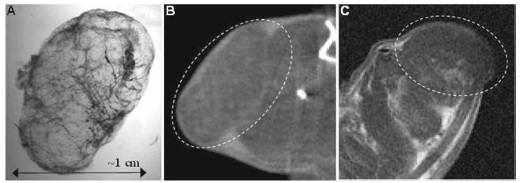
\includegraphics[scale=1]{intro_img/Oldham_2006_tumourstaining.jpg}
		\caption{Figure showing the advantage of optical CT imaging over other modalities. Part (A) shows a projection image of a HCT116 tumour after optical clearing. (B) is an \textit{in vivo} $\mu$-CT image of the same tumour with 50$\mu$m resolution. (C) is \textit{in vivo} T1 weighted contrast enhanced $\mu$-MRI image of a similar tumour. The superior resolution and contrast in the optical CT image is evident. Images  adapted from \cite{Oldham:2006}.}
		\label{fig:tumourstaining}
	\end{figure}
	
	
	
	
	
	\newpage
	\section{Conclusions}
	
	There is significant potential for further development of optical CT. Some new ideas include time-gating OPT using non-linear optics \cite{Bassi:2010}. Up-conversion using a crystal and Ti:sapphire laser  selects only ballistic light,  reducing scattering artefacts. However, employing this technique would significantly increase the system cost and complexity.
	
	Another group have successfully combined fluorescence lifetime imaging microscopy (FLIM) 
	with OPT \cite{McGinty:2008ix}. FLIM, a ratiometric modality, can provide quantitative information about the local environment around fluorophores including pH, temperature and refractive index. Protein-protein interactions can be probed using F\"{o}rster  resonance energy transfer (FRET) which can be measured using FLIM.  The set-up for FLIM-OPT is very similar to OPT and  a mathematical model is required to calculate fluorescence lifetimes from projection data. Projections are recorded for a series of time-delays for each angle. \textit{In vivo} FLIM OPT has also been reported \cite{McGinty:2011vm}, and these methods could possibly be very useful for drug screening, espcially using FRET. The authors note that using a modulated CMOS camera and sinusoidally varying LED source could be a cheaper way of implementing FLIM-OPT \cite{McGinty:2011vm}.
	
	Other improvements include the development of a computational techniques leading to increased sensitivity \cite{Hornblad:2011fh}. This is an adaptation of histogram equalisation, an established technique.
	The modulation transfer function (MTF), commonly used in optics as a measure of resolution, has been used to improve filtered in FBP \cite{Chen:2012}.
	An established technique of high dynamic range imaging has been applied to optical CT on several occasions and most recently by Fei \textit{et al.} in 2012 \cite{Peng:2012wi}.
	
	A potentially improved version of OptECT has been reported by Lorbeer \textit{et al.} in 2011  \cite{Lorbeer:2011}. A first generation scanning laser set-up is used to record fluorescent signal giving a hundredfold increase in photon collection efficiency over CCD-based set-ups. 
	
	The  biological benefits of all these new techniques have not been fully explored and there is still plenty of scope for improving this new modality.  Overall, it appears optical CT could be the ideal modality to help us understand the biological origin of contrast in MR images. Although optical CT itself will probably never be used clinically, due to the limit on sample sizes, we hope that it can help increase the usefulness of MRI. There is also potential for optical CT to be used in pre-clinical screening of drugs and in monitoring tumour progression. Especially exciting is the possibility of using fluorescent proteins to track interactions between tumour and host cells. 
	
	


